% ======================================================================
%  Somantha Manuranga - Master-Lebenslauf (Deutsch)
%
%  Dies ist die MASTER-Version mit allen Stationen und Projekten. Für
%  eine konkrete Bewerbung die Datei kopieren und Projekte und Zeilen
%  streichen, die nicht zur Stellenanzeige passen (Ziel: zwei Seiten).
%
%  Build:  pdflatex cv-de.tex   (zweimal, wegen der Seitenzahl)
%   oder:  npm run cv           (im Hauptordner; erzeugt EN + DE)
%  Layout und persönliche Daten: cv-style.tex
%  Hinweis: Kein gerades Anführungszeichen (") im Text verwenden.
% ======================================================================
\documentclass[a4paper,10pt]{article}

\newcommand{\cvlang}{ngerman}
\newcommand{\cvpdflang}{de-DE}
\newcommand{\cvdoctitle}{Lebenslauf}
\newcommand{\cvpageword}{Seite}
% ======================================================================
%  Shared style for the master CV (cv-en.tex and cv-de.tex)
%
%  Layout follows the previous CV (Jake Gutierrez's resume template, MIT
%  licence), adapted to A4 and tuned for applicant tracking systems (ATS):
%    - one column, standard section names, real text only
%    - no icon fonts (they extract as garbage characters)
%    - every glyph mapped to Unicode, f-ligatures switched off
%    - PDF title, author and keywords set
%
%  Before % ======================================================================
%  Shared style for the master CV (cv-en.tex and cv-de.tex)
%
%  Layout follows the previous CV (Jake Gutierrez's resume template, MIT
%  licence), adapted to A4 and tuned for applicant tracking systems (ATS):
%    - one column, standard section names, real text only
%    - no icon fonts (they extract as garbage characters)
%    - every glyph mapped to Unicode, f-ligatures switched off
%    - PDF title, author and keywords set
%
%  Before % ======================================================================
%  Shared style for the master CV (cv-en.tex and cv-de.tex)
%
%  Layout follows the previous CV (Jake Gutierrez's resume template, MIT
%  licence), adapted to A4 and tuned for applicant tracking systems (ATS):
%    - one column, standard section names, real text only
%    - no icon fonts (they extract as garbage characters)
%    - every glyph mapped to Unicode, f-ligatures switched off
%    - PDF title, author and keywords set
%
%  Before \input{cv-style} the main file must define:
%    \cvlang      babel language (english or ngerman)
%    \cvpdflang   PDF language tag (en-GB or de-DE)
%    \cvdoctitle  document title for the PDF metadata
%    \cvpageword  the word for "page" in the footer
% ======================================================================

\usepackage[T1]{fontenc}
\usepackage[utf8]{inputenc}
\usepackage[\cvlang]{babel}
\usepackage{lmodern}
\usepackage[a4paper,left=1.45cm,right=1.45cm,top=1.1cm,bottom=1.45cm,footskip=0.7cm]{geometry}
\usepackage{titlesec}
\usepackage{enumitem}
\usepackage{graphicx}
\usepackage{xcolor}
\usepackage{fancyhdr}
\usepackage{lastpage}
\usepackage{microtype}
\usepackage[hidelinks]{hyperref}

% ---------- ATS: machine-readable text ----------
\input{glyphtounicode}
\pdfgentounicode=1
\DisableLigatures[f]{encoding = *, family = *}

% ---------- Personal data (edit once, used by both languages) ----------
\newcommand{\cvname}{Somantha Manuranga}
\newcommand{\cvphone}{+49 174 7656939}
\newcommand{\cvemail}{somanthamanuranga@gmail.com}
\newcommand{\cvlinkedin}{linkedin.com/in/somantha-manuranga-b73432192}
\newcommand{\cvgithub}{github.com/SomanthaManuranga}
\newcommand{\cvportfolio}{somanthamanuranga.github.io/portfolio}

% Set to \photofalse for a version without a photo (some online
% application forms and international employers prefer that).
\newif\ifphoto
\phototrue

\hypersetup{
  pdftitle={\cvname\ - \cvdoctitle},
  pdfauthor={\cvname},
  pdfsubject={\cvdoctitle},
  pdfkeywords={AI Engineer, Machine Learning, Deep Learning, Computer Vision, NLP, LLM, PyTorch, Python, Industrial AI, Werkstudent},
  pdflang={\cvpdflang},
}

% ---------- Page ----------
\pagestyle{fancy}
\fancyhf{}
\renewcommand{\headrulewidth}{0pt}
\renewcommand{\footrulewidth}{0pt}
\fancyfoot[C]{\footnotesize\color{black!55}\cvname\ \textperiodcentered\ \cvpageword\ \thepage\ / \pageref*{LastPage}}
\setlength{\parindent}{0pt}
\setlength{\tabcolsep}{0pt}
\raggedbottom
\raggedright
\urlstyle{same}

% ---------- Section headings: small caps with a rule ----------
\titleformat{\section}{\vspace{-5pt}\scshape\raggedright\large}{}{0em}{}[\color{black}\titlerule\vspace{-5pt}]
\titlespacing*{\section}{0pt}{9pt}{7pt}

% ---------- Building blocks ----------
% \cvheader{line 1}{line 2}{line 3}{line 4}
% Each contact detail sits in an \mbox so that it is never hyphenated or
% split across lines (a broken email address or URL confuses ATS parsers).
\newcommand{\cvheader}[4]{%
  \begin{minipage}[c]{0.78\textwidth}
    {\Huge\bfseries \cvname}\\[6pt]
    {\small #1}\\[1.5pt]
    {\small #2}\\[1.5pt]
    {\small #3}\\[1.5pt]
    {\small #4}
  \end{minipage}%
  \hfill
  \ifphoto
  \begin{minipage}[c]{0.19\textwidth}
    \raggedleft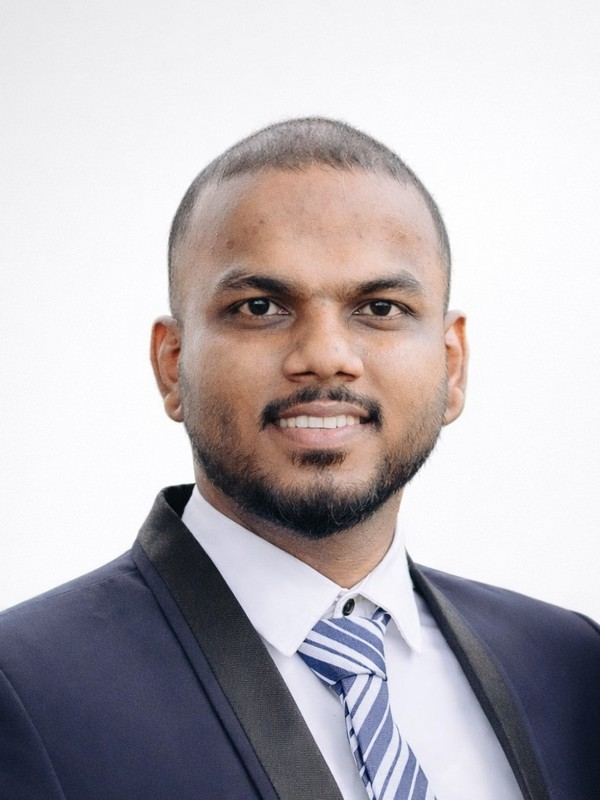
\includegraphics[width=2.75cm]{photo.jpg}
  \end{minipage}%
  \fi
  \par\vspace{3pt}
}
\newcommand{\cvsep}{\hspace{5pt}\textbullet\hspace{5pt}}

% Entry lists
\newcommand{\cvliststart}{\begin{itemize}[leftmargin=0.25cm, label={}, itemsep=3pt, topsep=0pt, parsep=0pt]}
\newcommand{\cvlistend}{\end{itemize}}

% \cventry{organisation}{location}{role or degree}{dates}
\newcommand{\cventry}[4]{%
  \item
  \begin{tabular*}{\linewidth}[t]{l@{\extracolsep{\fill}}r}
    \textbf{#1} & {\small #2} \\
    \textit{\small #3} & \textit{\small #4} \\
  \end{tabular*}\nopagebreak\vspace{-2pt}
}

% \cvproject{name}{technologies}{year}
\newcommand{\cvproject}[3]{%
  \item
  \begin{tabular*}{\linewidth}[t]{l@{\extracolsep{\fill}}r}
    {\small\textbf{#1} $|$ \textit{#2}} & \textit{\small #3} \\
  \end{tabular*}\nopagebreak\vspace{-2pt}
}

% \cvgroup{label}: sub-heading inside the project list
\newcommand{\cvgroup}[1]{\item[] \vspace{1pt}{\small\bfseries\itshape #1}\vspace{-1pt}}

% Bullet points under an entry
\newcommand{\cvpointsstart}{\begin{itemize}[leftmargin=0.45cm, label=\textbullet, itemsep=0.5pt, topsep=1pt, parsep=0pt]\small}
\newcommand{\cvpointsend}{\end{itemize}}

% \cvline{label}{text}: one line in the skills-style sections
\newcommand{\cvline}[2]{\item {\small \textbf{#1:} #2}}
 the main file must define:
%    \cvlang      babel language (english or ngerman)
%    \cvpdflang   PDF language tag (en-GB or de-DE)
%    \cvdoctitle  document title for the PDF metadata
%    \cvpageword  the word for "page" in the footer
% ======================================================================

\usepackage[T1]{fontenc}
\usepackage[utf8]{inputenc}
\usepackage[\cvlang]{babel}
\usepackage{lmodern}
\usepackage[a4paper,left=1.45cm,right=1.45cm,top=1.1cm,bottom=1.45cm,footskip=0.7cm]{geometry}
\usepackage{titlesec}
\usepackage{enumitem}
\usepackage{graphicx}
\usepackage{xcolor}
\usepackage{fancyhdr}
\usepackage{lastpage}
\usepackage{microtype}
\usepackage[hidelinks]{hyperref}

% ---------- ATS: machine-readable text ----------
\input{glyphtounicode}
\pdfgentounicode=1
\DisableLigatures[f]{encoding = *, family = *}

% ---------- Personal data (edit once, used by both languages) ----------
\newcommand{\cvname}{Somantha Manuranga}
\newcommand{\cvphone}{+49 174 7656939}
\newcommand{\cvemail}{somanthamanuranga@gmail.com}
\newcommand{\cvlinkedin}{linkedin.com/in/somantha-manuranga-b73432192}
\newcommand{\cvgithub}{github.com/SomanthaManuranga}
\newcommand{\cvportfolio}{somanthamanuranga.github.io/portfolio}

% Set to \photofalse for a version without a photo (some online
% application forms and international employers prefer that).
\newif\ifphoto
\phototrue

\hypersetup{
  pdftitle={\cvname\ - \cvdoctitle},
  pdfauthor={\cvname},
  pdfsubject={\cvdoctitle},
  pdfkeywords={AI Engineer, Machine Learning, Deep Learning, Computer Vision, NLP, LLM, PyTorch, Python, Industrial AI, Werkstudent},
  pdflang={\cvpdflang},
}

% ---------- Page ----------
\pagestyle{fancy}
\fancyhf{}
\renewcommand{\headrulewidth}{0pt}
\renewcommand{\footrulewidth}{0pt}
\fancyfoot[C]{\footnotesize\color{black!55}\cvname\ \textperiodcentered\ \cvpageword\ \thepage\ / \pageref*{LastPage}}
\setlength{\parindent}{0pt}
\setlength{\tabcolsep}{0pt}
\raggedbottom
\raggedright
\urlstyle{same}

% ---------- Section headings: small caps with a rule ----------
\titleformat{\section}{\vspace{-5pt}\scshape\raggedright\large}{}{0em}{}[\color{black}\titlerule\vspace{-5pt}]
\titlespacing*{\section}{0pt}{9pt}{7pt}

% ---------- Building blocks ----------
% \cvheader{line 1}{line 2}{line 3}{line 4}
% Each contact detail sits in an \mbox so that it is never hyphenated or
% split across lines (a broken email address or URL confuses ATS parsers).
\newcommand{\cvheader}[4]{%
  \begin{minipage}[c]{0.78\textwidth}
    {\Huge\bfseries \cvname}\\[6pt]
    {\small #1}\\[1.5pt]
    {\small #2}\\[1.5pt]
    {\small #3}\\[1.5pt]
    {\small #4}
  \end{minipage}%
  \hfill
  \ifphoto
  \begin{minipage}[c]{0.19\textwidth}
    \raggedleft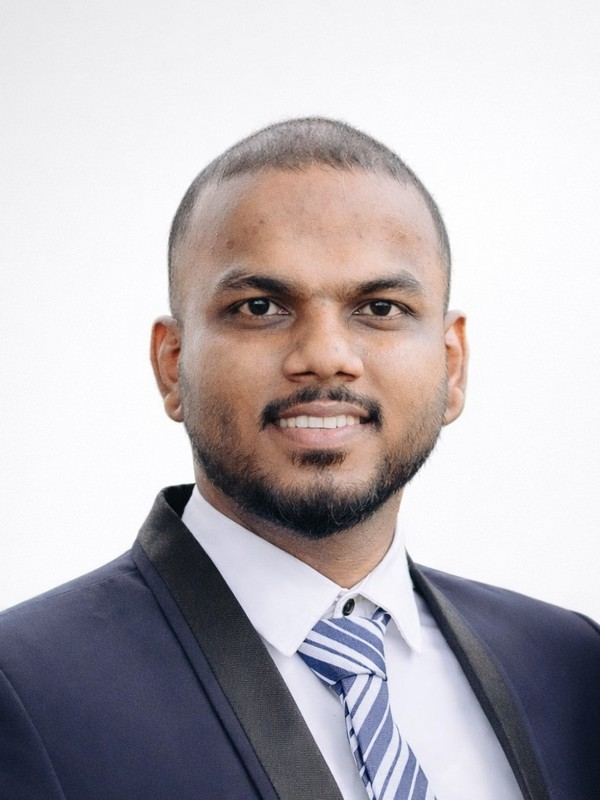
\includegraphics[width=2.75cm]{photo.jpg}
  \end{minipage}%
  \fi
  \par\vspace{3pt}
}
\newcommand{\cvsep}{\hspace{5pt}\textbullet\hspace{5pt}}

% Entry lists
\newcommand{\cvliststart}{\begin{itemize}[leftmargin=0.25cm, label={}, itemsep=3pt, topsep=0pt, parsep=0pt]}
\newcommand{\cvlistend}{\end{itemize}}

% \cventry{organisation}{location}{role or degree}{dates}
\newcommand{\cventry}[4]{%
  \item
  \begin{tabular*}{\linewidth}[t]{l@{\extracolsep{\fill}}r}
    \textbf{#1} & {\small #2} \\
    \textit{\small #3} & \textit{\small #4} \\
  \end{tabular*}\nopagebreak\vspace{-2pt}
}

% \cvproject{name}{technologies}{year}
\newcommand{\cvproject}[3]{%
  \item
  \begin{tabular*}{\linewidth}[t]{l@{\extracolsep{\fill}}r}
    {\small\textbf{#1} $|$ \textit{#2}} & \textit{\small #3} \\
  \end{tabular*}\nopagebreak\vspace{-2pt}
}

% \cvgroup{label}: sub-heading inside the project list
\newcommand{\cvgroup}[1]{\item[] \vspace{1pt}{\small\bfseries\itshape #1}\vspace{-1pt}}

% Bullet points under an entry
\newcommand{\cvpointsstart}{\begin{itemize}[leftmargin=0.45cm, label=\textbullet, itemsep=0.5pt, topsep=1pt, parsep=0pt]\small}
\newcommand{\cvpointsend}{\end{itemize}}

% \cvline{label}{text}: one line in the skills-style sections
\newcommand{\cvline}[2]{\item {\small \textbf{#1:} #2}}
 the main file must define:
%    \cvlang      babel language (english or ngerman)
%    \cvpdflang   PDF language tag (en-GB or de-DE)
%    \cvdoctitle  document title for the PDF metadata
%    \cvpageword  the word for "page" in the footer
% ======================================================================

\usepackage[T1]{fontenc}
\usepackage[utf8]{inputenc}
\usepackage[\cvlang]{babel}
\usepackage{lmodern}
\usepackage[a4paper,left=1.45cm,right=1.45cm,top=1.1cm,bottom=1.45cm,footskip=0.7cm]{geometry}
\usepackage{titlesec}
\usepackage{enumitem}
\usepackage{graphicx}
\usepackage{xcolor}
\usepackage{fancyhdr}
\usepackage{lastpage}
\usepackage{microtype}
\usepackage[hidelinks]{hyperref}

% ---------- ATS: machine-readable text ----------
\input{glyphtounicode}
\pdfgentounicode=1
\DisableLigatures[f]{encoding = *, family = *}

% ---------- Personal data (edit once, used by both languages) ----------
\newcommand{\cvname}{Somantha Manuranga}
\newcommand{\cvphone}{+49 174 7656939}
\newcommand{\cvemail}{somanthamanuranga@gmail.com}
\newcommand{\cvlinkedin}{linkedin.com/in/somantha-manuranga-b73432192}
\newcommand{\cvgithub}{github.com/SomanthaManuranga}
\newcommand{\cvportfolio}{somanthamanuranga.github.io/portfolio}

% Set to \photofalse for a version without a photo (some online
% application forms and international employers prefer that).
\newif\ifphoto
\phototrue

\hypersetup{
  pdftitle={\cvname\ - \cvdoctitle},
  pdfauthor={\cvname},
  pdfsubject={\cvdoctitle},
  pdfkeywords={AI Engineer, Machine Learning, Deep Learning, Computer Vision, NLP, LLM, PyTorch, Python, Industrial AI, Werkstudent},
  pdflang={\cvpdflang},
}

% ---------- Page ----------
\pagestyle{fancy}
\fancyhf{}
\renewcommand{\headrulewidth}{0pt}
\renewcommand{\footrulewidth}{0pt}
\fancyfoot[C]{\footnotesize\color{black!55}\cvname\ \textperiodcentered\ \cvpageword\ \thepage\ / \pageref*{LastPage}}
\setlength{\parindent}{0pt}
\setlength{\tabcolsep}{0pt}
\raggedbottom
\raggedright
\urlstyle{same}

% ---------- Section headings: small caps with a rule ----------
\titleformat{\section}{\vspace{-5pt}\scshape\raggedright\large}{}{0em}{}[\color{black}\titlerule\vspace{-5pt}]
\titlespacing*{\section}{0pt}{9pt}{7pt}

% ---------- Building blocks ----------
% \cvheader{line 1}{line 2}{line 3}{line 4}
% Each contact detail sits in an \mbox so that it is never hyphenated or
% split across lines (a broken email address or URL confuses ATS parsers).
\newcommand{\cvheader}[4]{%
  \begin{minipage}[c]{0.78\textwidth}
    {\Huge\bfseries \cvname}\\[6pt]
    {\small #1}\\[1.5pt]
    {\small #2}\\[1.5pt]
    {\small #3}\\[1.5pt]
    {\small #4}
  \end{minipage}%
  \hfill
  \ifphoto
  \begin{minipage}[c]{0.19\textwidth}
    \raggedleft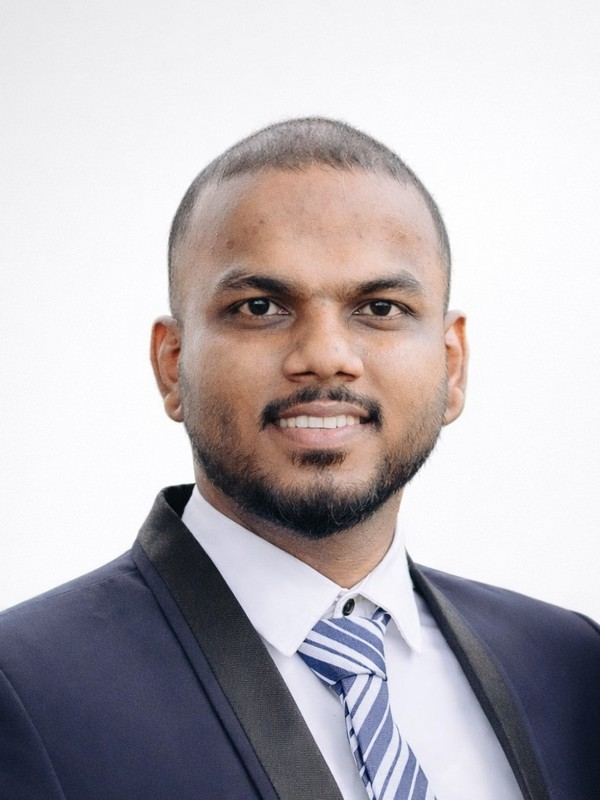
\includegraphics[width=2.75cm]{photo.jpg}
  \end{minipage}%
  \fi
  \par\vspace{3pt}
}
\newcommand{\cvsep}{\hspace{5pt}\textbullet\hspace{5pt}}

% Entry lists
\newcommand{\cvliststart}{\begin{itemize}[leftmargin=0.25cm, label={}, itemsep=3pt, topsep=0pt, parsep=0pt]}
\newcommand{\cvlistend}{\end{itemize}}

% \cventry{organisation}{location}{role or degree}{dates}
\newcommand{\cventry}[4]{%
  \item
  \begin{tabular*}{\linewidth}[t]{l@{\extracolsep{\fill}}r}
    \textbf{#1} & {\small #2} \\
    \textit{\small #3} & \textit{\small #4} \\
  \end{tabular*}\nopagebreak\vspace{-2pt}
}

% \cvproject{name}{technologies}{year}
\newcommand{\cvproject}[3]{%
  \item
  \begin{tabular*}{\linewidth}[t]{l@{\extracolsep{\fill}}r}
    {\small\textbf{#1} $|$ \textit{#2}} & \textit{\small #3} \\
  \end{tabular*}\nopagebreak\vspace{-2pt}
}

% \cvgroup{label}: sub-heading inside the project list
\newcommand{\cvgroup}[1]{\item[] \vspace{1pt}{\small\bfseries\itshape #1}\vspace{-1pt}}

% Bullet points under an entry
\newcommand{\cvpointsstart}{\begin{itemize}[leftmargin=0.45cm, label=\textbullet, itemsep=0.5pt, topsep=1pt, parsep=0pt]\small}
\newcommand{\cvpointsend}{\end{itemize}}

% \cvline{label}{text}: one line in the skills-style sections
\newcommand{\cvline}[2]{\item {\small \textbf{#1:} #2}}


\begin{document}

% ---------------------------------------------------------------- KOPF
\cvheader
  {Amberg, Deutschland \cvsep Nationalität: sri-lankisch \cvsep Telefon: \mbox{\cvphone}}
  {E-Mail: \mbox{\href{mailto:\cvemail}{\cvemail}} \cvsep GitHub: \mbox{\href{https://\cvgithub}{\cvgithub}}}
  {LinkedIn: \mbox{\href{https://www.\cvlinkedin}{\cvlinkedin}}}
  {Portfolio: \mbox{\href{https://\cvportfolio/}{\cvportfolio}}}

% -------------------------------------------------------------- PROFIL
\section{Profil}
{\small
AI Engineer und Masterstudent im Studiengang Artificial Intelligence for Industrial Applications mit Bachelorabschluss
im Maschinenbau. Werkstudent für KI und Automatisierung bei der syskomp gehmeyr GmbH, zuvor Berufserfahrung in der
Luftfahrtkonstruktion und Produktionsautomatisierung. Schwerpunkte: Computer Vision, LLMs/NLP und Machine Learning
für industrielle Prozesse. Sicher in Python und PyTorch, mit Fokus auf sorgfältige Evaluierung und Modelle, die sich
produktiv einsetzen lassen (ONNX-Export, regelbasierte Edge-Modelle, kleine GPUs).
}

% ----------------------------------------------------- BERUFSERFAHRUNG
\section{Berufserfahrung}
\cvliststart

  \cventry{syskomp gehmeyr GmbH}{Amberg, Deutschland}
          {Werkstudent KI und Automatisierung, Teilzeit}{10/2026 -- heute}
  \cvpointsstart
    \item Anwendung von KI-Methoden auf Engineering- und Industrieprozesse im Maschinenbauumfeld.
    \item Entwicklung und Evaluierung von Python-Prototypen mit Fokus auf nachvollziehbare, validierte Ergebnisse.
    \item Zusammenarbeit mit den Fachabteilungen, um Anforderungen in praxistaugliche KI-Werkzeuge umzusetzen.
  \cvpointsend

  \cventry{KNSI Aviation Engineering}{Negombo, Sri Lanka}
          {Design Engineer (Konstruktionsingenieur), Vollzeit}{08/2023 -- 09/2024}
  \cvpointsstart
    \item Pflege von Compliance-Daten und technischer Dokumentation mit SQL und Excel nach Luftfahrtstandards.
    \item Automatisierte SQL-/Excel-Berichtsvorlagen entwickelt; wöchentlichen Reporting-Aufwand um 30\,\% reduziert.
    \item Produktionsdaten analysiert und Abläufe optimiert; Prozesseffizienz um 40\,\% gesteigert.
    \item Digitalisierung der Altdokumentation für schnelleren abteilungsübergreifenden Datenzugriff geleitet.
  \cvpointsend

  \cventry{CBL Group (Ceylon Biscuits Limited)}{Pannipitiya, Sri Lanka}
          {Praktikant (Internship Trainee), Mechatronik \& Daten}{02/2022 -- 11/2022}
  \cvpointsstart
    \item Mitarbeit an der Prozessoptimierung durch datengetriebene Lösungen und Automatisierungsprojekte.
    \item Unterstützung der End-of-Line-Automatisierung mit Knickarm- und Parallelrobotern.
    \item 3D-gedruckte Automatisierungskomponenten konstruiert und gefertigt; Beschaffungskosten und Lieferzeiten gesenkt.
    \item IoT-Sensoren zur Echtzeitüberwachung von Produktionsanlagen als Grundlage für Predictive Maintenance eingesetzt.
  \cvpointsend

\cvlistend

% --------------------------------------------------------- BILDUNGSWEG
\section{Bildungsweg}
\cvliststart

  \cventry{OTH Amberg-Weiden (Ostbayerische Technische Hochschule)}{Amberg, Deutschland}
          {M.Sc.\ Artificial Intelligence for Industrial Applications}{03/2025 -- heute (Abschluss vorauss.\ 2027)}
  \cvpointsstart
    \item Module: Computer Vision, Deep Vision, Deep Learning, NLP \& Information Retrieval, Autonome Robotik,
          AI Security \& Privacy, Machine Learning, Industrie 4.0.
  \cvpointsend

  \cventry{Vorbereitung auf das Masterstudium in Deutschland}{Sri Lanka / Deutschland}
          {Visumverfahren, Umzug und Deutschkurs}{10/2024 -- 02/2025}

  \cventry{University of Sri Jayewardenepura}{Sri Lanka}
          {B.Sc.\ (Hons) Maschinenbau, Nebenfach Mechatronik \textup{(GPA 3,27 / 4,0)}}{11/2019 -- 05/2023}
  \cvpointsstart
    \item Abschlussarbeit: CNN-Surrogatmodell zur Vorhersage des aerodynamischen Widerstands von 2D-Geometrien aus
          Bildern (ersetzt CFD-Simulationen).
    \item Projekt: Konstruktion und Bau eines CoreXY-3D-Druckers (mechanisches Design und Machine Learning).
  \cvpointsend

\cvlistend

% ------------------------------------------------------ FACHKENNTNISSE
\section{Fachkenntnisse}
\cvliststart
  \cvline{Programmierung \& Tools}{Python (fortgeschritten), C++, SQL, Git/GitHub, REST-APIs, pytest, LaTeX}
  \cvline{ML \& Deep Learning}{PyTorch, TensorFlow/Keras, scikit-learn, XGBoost, LightGBM, CatBoost, Optuna, CNN, RNN}
  \cvline{Computer Vision}{OpenCV, YOLOv8, Objekterkennung, semantische Segmentierung (U-Net, DeepLabV3+), Vision Transformers, Grad-CAM, ONNX}
  \cvline{NLP \& generative KI}{Hugging Face Transformers, LLMs (Qwen, Llama, GPT), Fine-Tuning (LoRA/PEFT), RAG, LangChain, agentische Workflows, SciBERT, LayoutLMv3, Tesseract OCR}
  \cvline{Robotik \& Industrie 4.0}{Webots, SLAM, Pfadplanung (A*), PID-Regelung, MQTT, digitale Zwillinge, IoT}
  \cvline{Daten \& Backend}{pandas, NumPy, Matplotlib, Seaborn, MongoDB, Power BI, ETL-Pipelines, Weights \& Biases}
  \cvline{Maschinenbau}{CAD/CAM, SolidWorks, CFD-Simulation, 3D-Druck, Mechatronik}
\cvlistend

% ------------------------------------------------------------ PROJEKTE
\section{Projekte}
\cvliststart

  \cvgroup{Industrielle KI \& Computer Vision}

  \cvproject{Fehlererkennung in Röntgenbildern von Gussteilen}{YOLOv8, OpenCV, ONNX}{2026}
  \cvpointsstart
    \item YOLOv8n zur Erkennung von Poren, Einschlüssen und Lunkern in GDXray-Röntgenbildern von Aluminiumguss
          trainiert (Split auf Serienebene): Test-mAP50 0,545, Precision 0,748.
    \item Fehleranalyse nach Defektgröße und CLAHE-Ablation; ONNX-Export mit identischen Detektionen (60 ms/Bild, CPU).
  \cvpointsend

  \cvproject{Korrosionssegmentierung: U-Net vs. DeepLabV3+}{PyTorch, segmentation-models-pytorch}{2026}
  \cvpointsstart
    \item Pixelgenaue Segmentierung von vier Korrosionszuständen auf Fotos von Stahlbrücken: mittlere IoU 0,523;
          U-Net ist bei der sicherheitskritischen Klasse \glqq Severe\grqq{} deutlich besser (IoU 0,325 vs. 0,266).
  \cvpointsend

  \cvproject{CNN-Surrogatmodell für den Luftwiderstand (Bachelorarbeit)}{TensorFlow, Keras, CFD}{2023}
  \cvpointsstart
    \item CNN sagt den Widerstandsbeiwert von 2D-Geometrien aus Bildern in Millisekunden statt per CFD-Simulation
          vorher; trainiert mit 12.000 simulierten Formen nach Vergleich von 7 Architekturen (Validierungs-MSE 0,0017).
    \item 0,06--2,77\,\% relativer Fehler bei unbekannten realen Formen inkl. NACA-Profilen (Referenz: SolidWorks).
  \cvpointsend

  \cvproject{Dashboard für industrielle Produktionskennzahlen}{Power BI, DAX, Power Query, SQL}{2025}
  \cvpointsstart
    \item Power-BI-Dashboards auf Basis von Sternschema-Modellen mit automatisierten ETL-Pipelines für Fertigungs-KPIs.
  \cvpointsend

  \cvproject{Stacking-Ensemble \& regelbasiertes Edge-Modell}{XGBoost, LightGBM, CatBoost, Optuna}{2025/26}
  \cvpointsstart
    \item Mit Optuna optimiertes Stacking-Ensemble mit R\textsuperscript{2} 0,848 bei 273 Merkmalen; drei
          If-else-Regeln (R\textsuperscript{2} 0,915) abgeleitet, die ohne ML-Bibliotheken auf einem Edge-Gerät laufen.
  \cvpointsend

  \cvproject{Pneumonie-Erkennung: CNN vs. ViT vs. Hybrid}{PyTorch, timm, Grad-CAM}{2026}
  \cvpointsstart
    \item ResNet-50, ViT-Base und TinyViT unter identischen Bedingungen verglichen (5-fach-CV-Ensembles): TinyViT
          erreicht 94,9\,\% Testgenauigkeit (F1 0,948); Aussagekraft der Grad-CAM-Erklärungen bewertet.
  \cvpointsend

  \cvproject{Simulation eines digitalen IR-Thermometers}{Python, NumPy, Signalverarbeitung}{2025}
  \cvpointsstart
    \item Physikbasierte Sensorsimulation (Rauschen, Drift, Emissionsgradfehler, Ausreißer) mit Filterung.
  \cvpointsend

  \cvgroup{LLMs, NLP \& Dokumenten-KI}

  \cvproject{Entfernen von Jailbreak-Backdoors aus LLMs}{PyTorch, Hugging Face, LoRA/PEFT}{2026}
  \cvpointsstart
    \item Bekannte Backdoor aus Qwen2.5-1.5B per hybridem Supervised Fine-Tuning mit vier Datengruppen auf einer
          8-GB-GPU entfernt: Angriffserfolgsrate von 95\,\% auf 1,7\,\% gesenkt bei 84\,\% Benign Accuracy.
    \item Mechanistische Analyse mit linearen Probes: Der Trigger wird weiterhin erkannt (ca. 97\,\%); die Abwehr
          ändert die Reaktion des Modells, löscht den Trigger aber nicht.
  \cvpointsend

  \cvproject{QuantumCircuit Dataset Builder}{SciBERT, Transformers, BeautifulSoup, PyMuPDF}{2025/26}
  \cvpointsstart
    \item Automatisierte Pipeline, die arXiv-Paper nach Quantenschaltkreis-Abbildungen durchsucht; SciBERT-Klassifikator
          für Bildunterschriften (F1 0,954) liefert 250 Metadatensätze und 160 extrahierte Bilder.
  \cvpointsend

  \cvproject{Formularverständnis mit LayoutLMv3}{LayoutLMv3, Hugging Face, Tesseract OCR}{2026}
  \cvpointsstart
    \item LayoutLMv3 für die Schlüssel-Wert-Extraktion aus gescannten Formularen (FUNSD) trainiert: F1 0,896.
  \cvpointsend

  \cvgroup{Robotik \& Industrie 4.0}

  \cvproject{Autonome Labyrinth-Navigation mit ROSbot}{Webots, SLAM, A*, PID, OpenCV}{2026}
  \cvpointsstart
    \item ROSbot erkundet unbekannte Labyrinthe mit LiDAR- und Tiefenkamera-Kartierung, Frontier Exploration,
          A*-Planung und PID-Regelung; 4 von 5 Labyrinthen vollständig gelöst, schnellster Lauf 54 Sekunden.
  \cvpointsend

  \cvproject{ALIA-Delivery: Digitaler Zwilling eines Klinikroboters}{Webots, MQTT, Flask, A*}{2025}
  \cvpointsstart
    \item Digitaler Zwilling einer Klinikstation (Teamprojekt): Ein TurtleBot3 erhält Lieferaufträge per MQTT von
          einem Flask-Leitstand, plant A*-Routen und fährt zum Patientenzimmer.
  \cvpointsend

  \cvproject{CoreXY-3D-Drucker}{Mechatronik, CAD/CAM, Firmware}{B.Sc.-Projekt}
  \cvpointsstart
    \item CoreXY-3D-Drucker von Grund auf konstruiert und gebaut: mechanisches Design, Kinematik und Firmware.
  \cvpointsend

  \cvgroup{Datenanalyse}

  \cvproject{Study Program Intelligence}{Python, pandas, Monte Carlo, MCDA}{2026}
  \cvpointsstart
    \item Reproduzierbare Analyse, welcher neue Studiengang die meisten Studierenden an die OTH Amberg-Weiden bringt:
          multikriterielle Entscheidungsanalyse unter Unsicherheit mit 10.000 Monte-Carlo-Ziehungen.
  \cvpointsend

  \cvproject{Social-Media-Nutzung von Studierenden: EDA}{pandas, Seaborn, Matplotlib}{2025}
  \cvpointsstart
    \item Explorative Analyse von 705 Studierenden aus 110 Ländern; Nutzungsdauer korreliert mit Schlaf (r = $-$0,79).
  \cvpointsend

\cvlistend

% --------------------------------------------------------- ZERTIFIKATE
\section{Weiterbildung \& Zertifikate}
\cvliststart
  \cvline{09/2025}{Bayerisch-Tschechische KI-Sommerschule, \glqq Controlling Robots with LLMs\grqq{} (32 Stunden), Speinshart}
  \cvline{DeepLearning.AI}{Deep Learning Specialization; Natural Language Processing Specialization (4 Kurse); AI for Medicine Specialization (3 Kurse)}
  \cvline{Vortrag}{\glqq Adaptive-RAG\grqq{} (NAACL-2024-Paper): 25-minütiger wissenschaftlicher Vortrag, Modul AI Conference, OTH Amberg-Weiden, Sommersemester 2026}
\cvlistend

% ------------------------------------------------------------ SPRACHEN
\section{Sprachen}
\cvliststart
  \item {\small \textbf{Englisch:} C1 (verhandlungssicher) \cvsep \textbf{Deutsch:} B1 (wird aktiv ausgebaut) \cvsep \textbf{Singhalesisch:} Muttersprache}
\cvlistend

% ---------------------------------------------------------- ENGAGEMENT
\section{Engagement \& Interessen}
\cvliststart
  \cvline{Unternehmertum}{VYROBA TECHS: CoreXY-3D-Drucker gebaut und in der Pandemie ein kleines Sonderteile-Geschäft betrieben}
  \cvline{Fußball}{Spieler beim FC Amberg; ehemaliger Kapitän der Fakultäts- und Universitätsmannschaft; University Colours Award 2022}
\cvlistend

\end{document}
